\chapter{Set-Up of Experiment}
To perform the experiment the items shown in \cref{fig:setup} are needed.
 \begin{figure}[H]
	\centering
	% \begin{framed}
	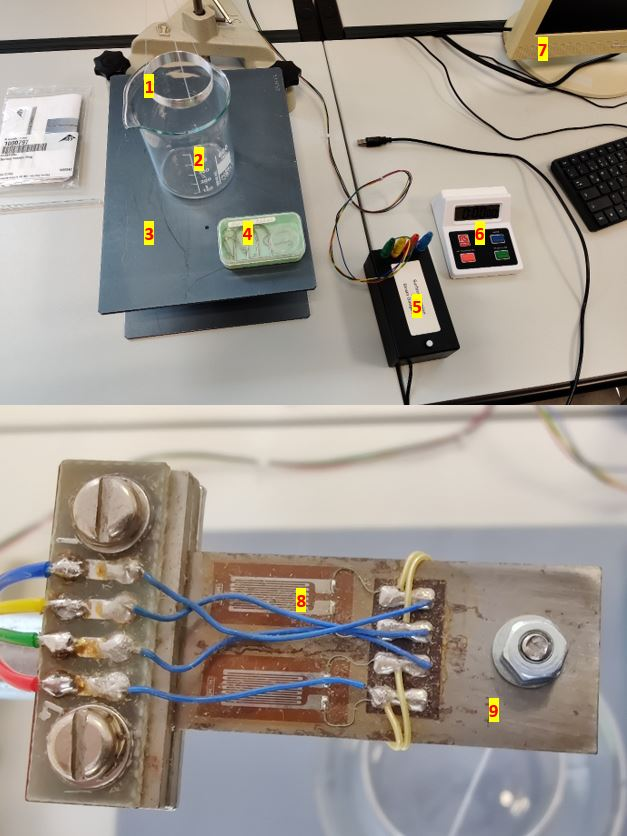
\includegraphics[width=.7\textwidth]{aufbau/Setup/setup_num}
	% \end{framed}
	%\includegraphics[width=12cm]{} % insert image (incl. numbering)
	\caption[Components needed for the experiment]{Components needed for the experiment. 1: \textsc{Du Noüy-ring}, 2: Glass beaker, 3: Lifting platform, 4: Calibration weights, 5: A/D converter box with offset button, 6: stopwatch, 7: Computer running \textsc{RealTerm}, 8: Strain gauges, 9: Cantilever.}
	\label{fig:setup}
\end{figure}

Using a desktop computer a serial connection via USB is established. A serial monitor - \textsc{RealTerm} - is used to log the inbound stream send by the MCU. The relevant settings are listed below:
\begin{itemize}
	\item 9600 Baud
	\item On the Display tab, \textit{ASCII} and \textit{New Line mode} are checked, \textit{Direct capture} remains
	un-checked.
	\item COM-Port as assigned by the OS.
\end{itemize}
The data is now continuously sent by the microcontroller. The data is displayed on the screen. A text file is created in which the data is written and saved. Three columns are displayed. The first column contains the time in seconds, the second the raw ADC data and the third column the filtered ADC data.\par
Now the setup is completed and the experiments can be started.
